\chapter*{Dibuja los circuitos lógicos para las siguientes expresiones}

Dibuja los circuitos lógicos para las siguientes expresiones:

\begin{enumerate}
    \item[(a)] $xyz \oplus x\overline{y}z$
    \item[(b)] $xy + x\overline{y}$
    \item[(c)] $xy\overline{z} + x\overline{yz}$
    \item[(d)] $\overline{x} + \overline{y} + xyz$
    
\end{enumerate}
 \begin{figure}[h!]
    \centering
    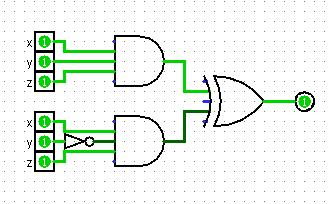
\includegraphics[width=\textwidth]{recursos/Ejercicio2/circuito_a.png}
    \caption{Circuito lógico para $xyz \oplus x\overline{y}z$}
\end{figure}
\newpage

\begin{figure}[h!]
    \centering
    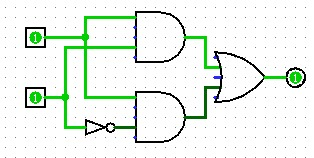
\includegraphics[width=\textwidth]{recursos/Ejercicio2/circuito_b.png}
    \caption{Circuito lógico para $xy + x\overline{y}$}
\end{figure}

\begin{figure}[h!]
    \centering
    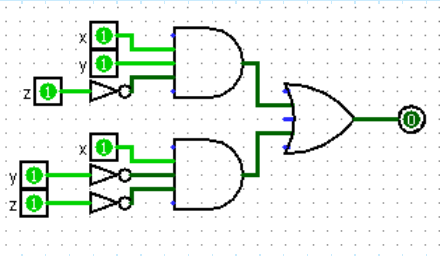
\includegraphics[width=\textwidth]{recursos/Ejercicio2/circuito_c.png}
    \caption{Circuito lógico para $xy\overline{z} + x\overline{yz}$}
\end{figure}

\begin{figure}[h!]
    \centering
    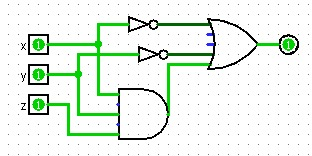
\includegraphics[width=\textwidth]{recursos/Ejercicio2/circuito_d.png}
    \caption{Circuito lógico para $\overline{x} + \overline{y} + xyz$}
\end{figure}



